\documentclass{standalone}
\usepackage{tikz}
\usetikzlibrary{patterns, positioning}
\usepackage[sfdefault]{ClearSans} %% option 'sfdefault' activates Clear Sans as the default text font
\usepackage[T1]{fontenc}

\begin{document}
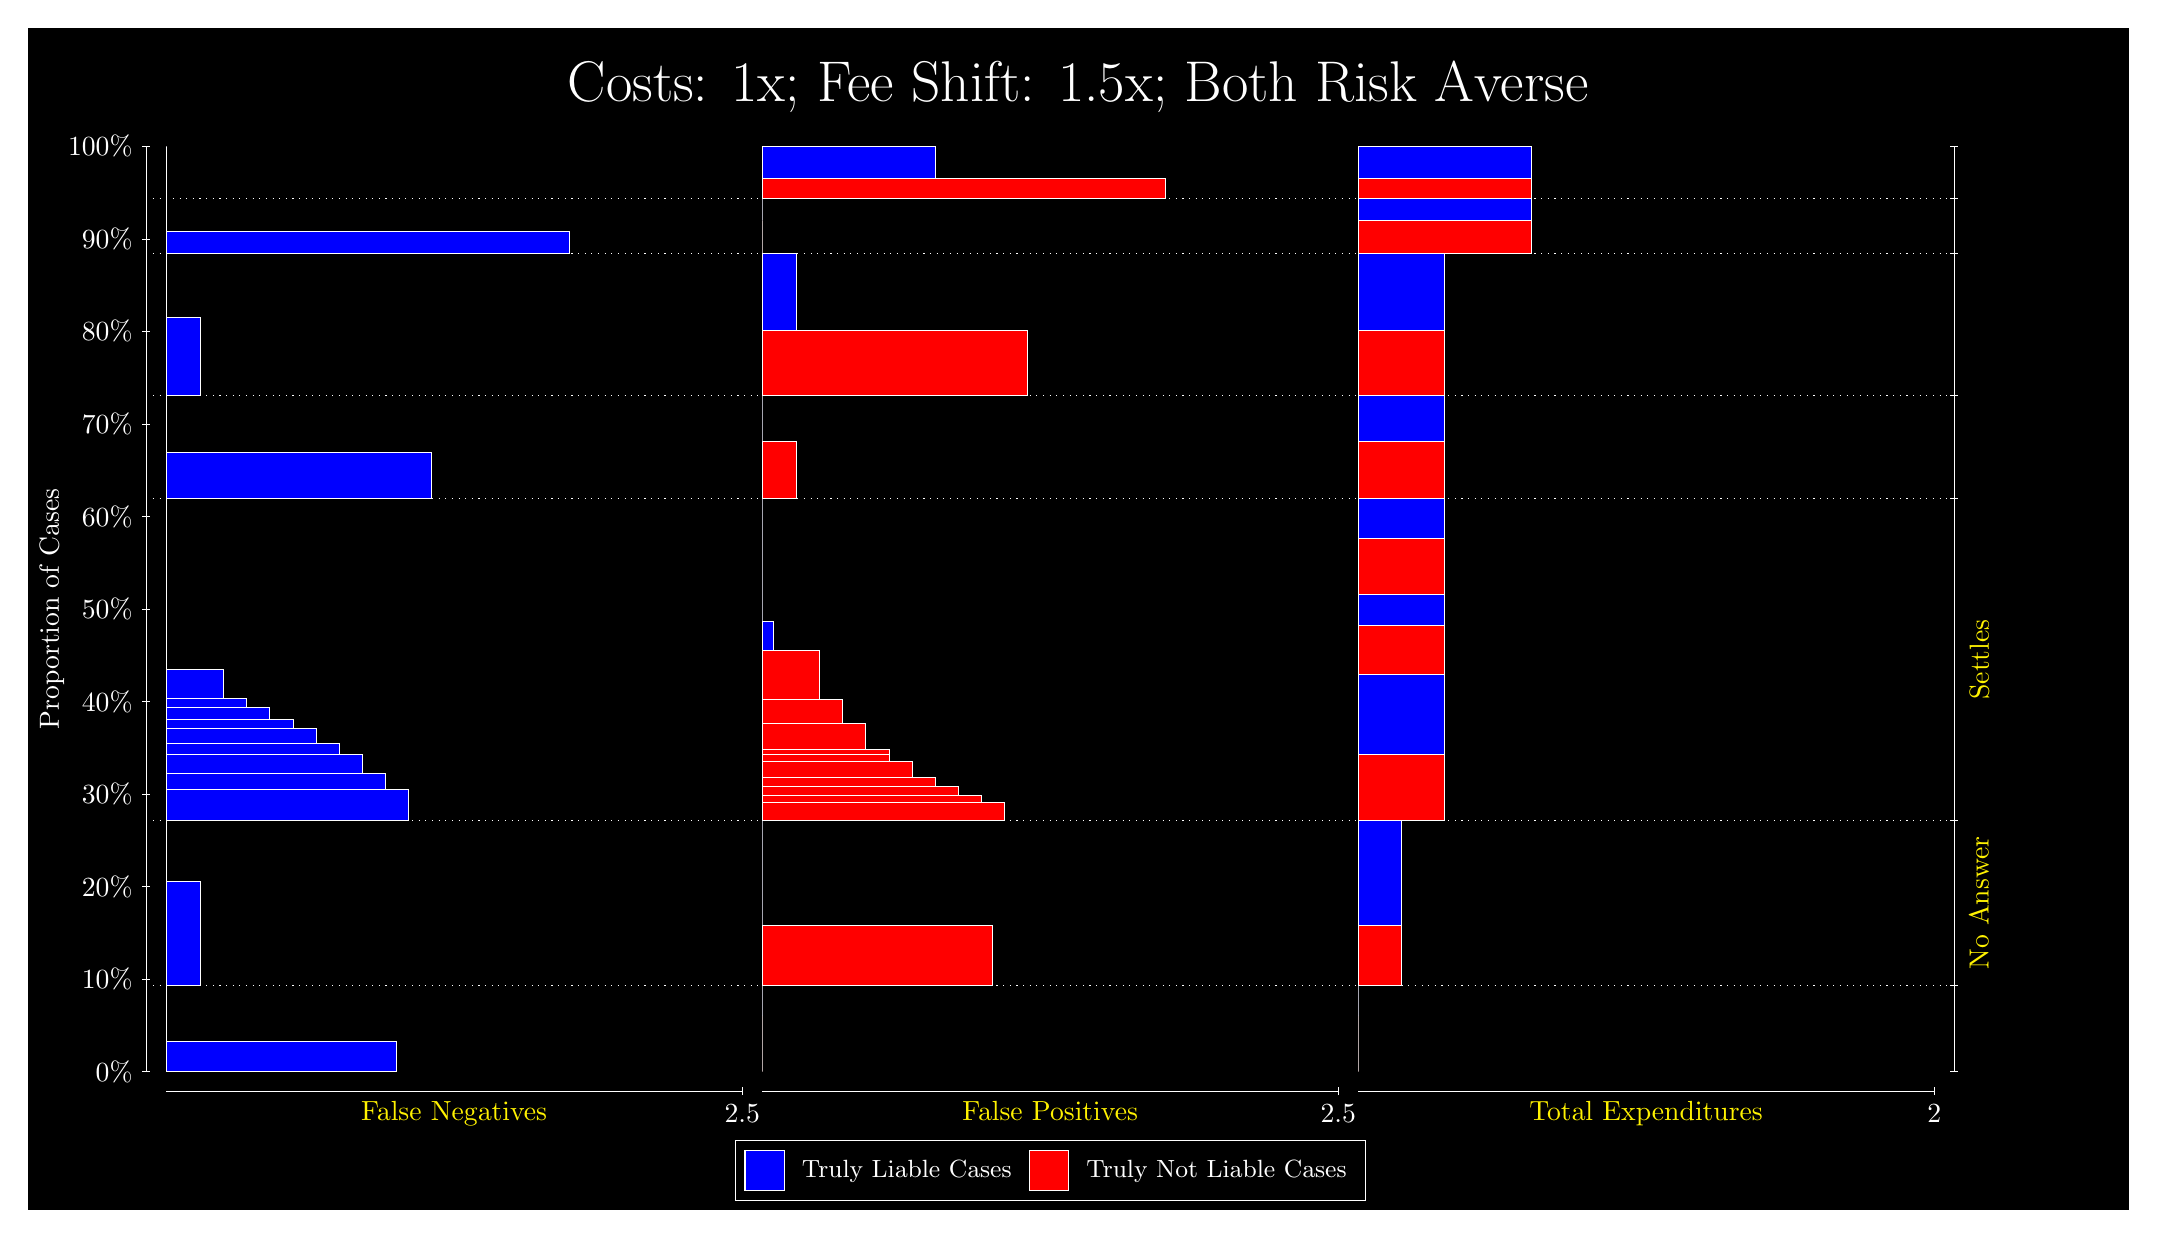
\begin{tikzpicture}
\draw[fill=black] (0,0) rectangle (26.667,15);
\draw[text=white] (0,13.5) rectangle (26.667,15) node[midway] {\huge Costs: 1x; Fee Shift: 1.5x; Both Risk Averse};
\draw[white, very thin] (1.5,1.75) -- (1.5,13.5);
\node[rotate=90, text=white, anchor=center] at (0.3, 7.625) {Proportion of Cases};
\draw[white, very thin] (1.45,1.75) -- (1.55,1.75);
\node[text=white, anchor=east] at (1.45, 1.75) {0\%};
\draw[white, very thin] (1.45,2.925) -- (1.55,2.925);
\node[text=white, anchor=east] at (1.45, 2.925) {10\%};
\draw[white, very thin] (1.45,4.1) -- (1.55,4.1);
\node[text=white, anchor=east] at (1.45, 4.1) {20\%};
\draw[white, very thin] (1.45,5.275) -- (1.55,5.275);
\node[text=white, anchor=east] at (1.45, 5.275) {30\%};
\draw[white, very thin] (1.45,6.45) -- (1.55,6.45);
\node[text=white, anchor=east] at (1.45, 6.45) {40\%};
\draw[white, very thin] (1.45,7.625) -- (1.55,7.625);
\node[text=white, anchor=east] at (1.45, 7.625) {50\%};
\draw[white, very thin] (1.45,8.8) -- (1.55,8.8);
\node[text=white, anchor=east] at (1.45, 8.8) {60\%};
\draw[white, very thin] (1.45,9.975) -- (1.55,9.975);
\node[text=white, anchor=east] at (1.45, 9.975) {70\%};
\draw[white, very thin] (1.45,11.15) -- (1.55,11.15);
\node[text=white, anchor=east] at (1.45, 11.15) {80\%};
\draw[white, very thin] (1.45,12.325) -- (1.55,12.325);
\node[text=white, anchor=east] at (1.45, 12.325) {90\%};
\draw[white, very thin] (1.45,13.5) -- (1.55,13.5);
\node[text=white, anchor=east] at (1.45, 13.5) {100\%};

\draw[white, very thin] (24.457,1.75) -- (24.457,13.5);
\draw[white, very thin] (24.407,1.75) -- (24.507,1.75);
\node[anchor=west] at (24.407, 1.75) {};
\draw[white, very thin] (24.407,2.8431) -- (24.507,2.8431);
\node[anchor=west] at (24.407, 2.8431) {};
\draw[white, very thin] (24.407,4.9348) -- (24.507,4.9348);
\node[anchor=west] at (24.407, 4.9348) {};
\draw[white, very thin] (24.407,9.0287) -- (24.507,9.0287);
\node[anchor=west] at (24.407, 9.0287) {};
\draw[white, very thin] (24.407,10.339) -- (24.507,10.339);
\node[anchor=west] at (24.407, 10.339) {};
\draw[white, very thin] (24.407,12.144) -- (24.507,12.144);
\node[anchor=west] at (24.407, 12.144) {};
\draw[white, very thin] (24.407,12.835) -- (24.507,12.835);
\node[anchor=west] at (24.407, 12.835) {};
\draw[white, very thin] (24.407,13.5) -- (24.507,13.5);
\node[anchor=west] at (24.407, 13.5) {};

\draw[white, very thin, fill=blue] (1.75,1.75) rectangle (4.6775,2.1352);
\draw[white, very thin, fill=red] (1.75,2.1352) rectangle (1.75,2.8431);
\draw[white, very thin, fill=blue] (1.75,2.8431) rectangle (2.1891,4.1648);
\draw[white, very thin, fill=red] (1.75,4.1648) rectangle (1.75,4.9348);
\draw[white, very thin, fill=blue] (1.75,4.9348) rectangle (4.8239,5.3359);
\draw[white, very thin, fill=blue] (1.75,5.3359) rectangle (4.5312,5.542);
\draw[white, very thin, fill=blue] (1.75,5.542) rectangle (4.2384,5.7811);
\draw[white, very thin, fill=blue] (1.75,5.7811) rectangle (3.9457,5.9161);
\draw[white, very thin, fill=blue] (1.75,5.9161) rectangle (3.6529,6.1128);
\draw[white, very thin, fill=blue] (1.75,6.1128) rectangle (3.3602,6.2242);
\draw[white, very thin, fill=blue] (1.75,6.2242) rectangle (3.0674,6.3701);
\draw[white, very thin, fill=blue] (1.75,6.3701) rectangle (2.7746,6.4934);
\draw[white, very thin, fill=blue] (1.75,6.4934) rectangle (2.4819,6.8616);
\draw[white, very thin, fill=red] (1.75,6.8616) rectangle (1.75,9.0287);
\draw[white, very thin, fill=blue] (1.75,9.0287) rectangle (5.1167,9.6131);
\draw[white, very thin, fill=red] (1.75,9.6131) rectangle (1.75,10.339);
\draw[white, very thin, fill=blue] (1.75,10.339) rectangle (2.1891,11.323);
\draw[white, very thin, fill=red] (1.75,11.323) rectangle (1.75,12.144);
\draw[white, very thin, fill=blue] (1.75,12.144) rectangle (6.8732,12.418);
\draw[white, very thin, fill=red] (1.75,12.418) rectangle (1.75,12.835);
\draw[white, very thin, fill=red] (1.75,12.835) rectangle (1.75,13.1);
\draw[white, very thin, fill=blue] (1.75,13.1) rectangle (1.75,13.5);
\draw[white, very thin, fill=red] (9.3189,1.75) rectangle (9.3189,2.4579);
\draw[white, very thin, fill=blue] (9.3189,2.4579) rectangle (9.3189,2.8431);
\draw[white, very thin, fill=red] (9.3189,2.8431) rectangle (12.246,3.6131);
\draw[white, very thin, fill=blue] (9.3189,3.6131) rectangle (9.3189,4.9348);
\draw[white, very thin, fill=red] (9.3189,4.9348) rectangle (12.393,5.1635);
\draw[white, very thin, fill=red] (9.3189,5.1635) rectangle (12.1,5.2562);
\draw[white, very thin, fill=red] (9.3189,5.2562) rectangle (11.807,5.3745);
\draw[white, very thin, fill=red] (9.3189,5.3745) rectangle (11.515,5.4807);
\draw[white, very thin, fill=red] (9.3189,5.4807) rectangle (11.222,5.6878);
\draw[white, very thin, fill=red] (9.3189,5.6878) rectangle (10.929,5.7728);
\draw[white, very thin, fill=red] (9.3189,5.7728) rectangle (10.929,5.8469);
\draw[white, very thin, fill=red] (9.3189,5.8469) rectangle (10.636,6.1707);
\draw[white, very thin, fill=red] (9.3189,6.1707) rectangle (10.344,6.4752);
\draw[white, very thin, fill=red] (9.3189,6.4752) rectangle (10.051,7.1019);
\draw[white, very thin, fill=blue] (9.3189,7.1019) rectangle (9.4652,7.4702);
\draw[white, very thin, fill=blue] (9.3189,7.4702) rectangle (9.3189,9.0287);
\draw[white, very thin, fill=red] (9.3189,9.0287) rectangle (9.758,9.7544);
\draw[white, very thin, fill=blue] (9.3189,9.7544) rectangle (9.3189,10.339);
\draw[white, very thin, fill=red] (9.3189,10.339) rectangle (12.686,11.16);
\draw[white, very thin, fill=blue] (9.3189,11.16) rectangle (9.758,12.144);
\draw[white, very thin, fill=red] (9.3189,12.144) rectangle (9.3189,12.561);
\draw[white, very thin, fill=blue] (9.3189,12.561) rectangle (9.3189,12.835);
\draw[white, very thin, fill=red] (9.3189,12.835) rectangle (14.442,13.1);
\draw[white, very thin, fill=blue] (9.3189,13.1) rectangle (11.515,13.5);
\draw[white, very thin, fill=red] (16.888,1.75) rectangle (16.888,2.4579);
\draw[white, very thin, fill=blue] (16.888,2.4579) rectangle (16.888,2.8431);
\draw[white, very thin, fill=red] (16.888,2.8431) rectangle (17.437,3.6131);
\draw[white, very thin, fill=blue] (16.888,3.6131) rectangle (17.437,4.9348);
\draw[white, very thin, fill=red] (16.888,4.9348) rectangle (17.986,5.7728);
\draw[white, very thin, fill=blue] (16.888,5.7728) rectangle (17.986,6.7896);
\draw[white, very thin, fill=red] (16.888,6.7896) rectangle (17.986,7.4163);
\draw[white, very thin, fill=blue] (16.888,7.4163) rectangle (17.986,7.8174);
\draw[white, very thin, fill=red] (16.888,7.8174) rectangle (17.986,8.5198);
\draw[white, very thin, fill=blue] (16.888,8.5198) rectangle (17.986,9.0287);
\draw[white, very thin, fill=red] (16.888,9.0287) rectangle (17.986,9.7544);
\draw[white, very thin, fill=blue] (16.888,9.7544) rectangle (17.986,10.339);
\draw[white, very thin, fill=red] (16.888,10.339) rectangle (17.986,11.16);
\draw[white, very thin, fill=blue] (16.888,11.16) rectangle (17.986,12.144);
\draw[white, very thin, fill=red] (16.888,12.144) rectangle (19.083,12.561);
\draw[white, very thin, fill=blue] (16.888,12.561) rectangle (19.083,12.835);
\draw[white, very thin, fill=red] (16.888,12.835) rectangle (19.083,13.1);
\draw[white, very thin, fill=blue] (16.888,13.1) rectangle (19.083,13.5);
\draw[white, dotted] (1.5,2.8431) -- (24.457,2.8431);
\draw[white, dotted] (1.5,4.9348) -- (24.457,4.9348);
\draw[white, dotted] (1.5,9.0287) -- (24.457,9.0287);
\draw[white, dotted] (1.5,10.339) -- (24.457,10.339);
\draw[white, dotted] (1.5,12.144) -- (24.457,12.144);
\draw[white, dotted] (1.5,12.835) -- (24.457,12.835);
\draw[white, very thin] (1.75,1.5) -- (9.0689,1.5);
\node[text=yellow, anchor=north] at (5.4094, 1.5) {False Negatives};
\draw[white, very thin] (9.0689,1.45) -- (9.0689,1.55);
\node[text=white, anchor=north] at (9.0689, 1.45) {2.5};

\draw[white, very thin] (9.3189,1.5) -- (16.638,1.5);
\node[text=yellow, anchor=north] at (12.978, 1.5) {False Positives};
\draw[white, very thin] (16.638,1.45) -- (16.638,1.55);
\node[text=white, anchor=north] at (16.638, 1.45) {2.5};

\draw[white, very thin] (16.888,1.5) -- (24.207,1.5);
\node[text=yellow, anchor=north] at (20.547, 1.5) {Total Expenditures};
\draw[white, very thin] (24.207,1.45) -- (24.207,1.55);
\node[text=white, anchor=north] at (24.207, 1.45) {2};


\node[text=yellow, centered, rotate=90] at (24.777, 3.8889) {No Answer};
\node[text=yellow, centered, rotate=90] at (24.777, 6.9818) {Settles};





\draw (12.978300999999998,1.5) node[draw=none] (baseCoordinate) {};
\begin{scope}[align=center]
        \matrix[scale=0.5, draw=white, below=0.5cm of baseCoordinate, nodes={draw}, column sep=0.1cm]{
            \node[rectangle, draw, minimum width=0.5cm, minimum height=0.5cm, fill=blue] {}; &
            \node[draw=none, font=\small, text=white] (B) {Truly Liable Cases}; &
            \node[rectangle, draw, minimum width=0.5cm, minimum height=0.5cm, fill=red] {}; &
            \node[draw=none, font=\small, text=white] (B) {Truly Not Liable Cases}; \\
            };
\end{scope}

\end{tikzpicture}
\end{document}